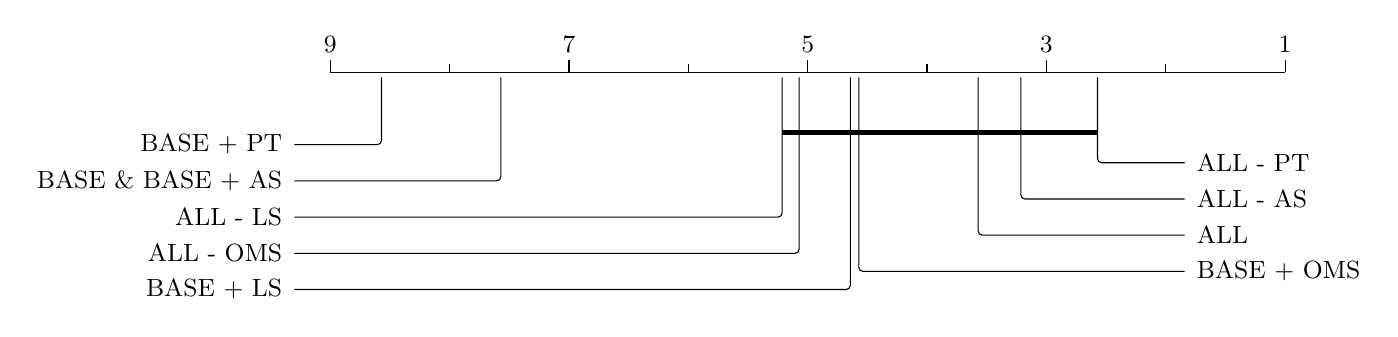
\begin{tikzpicture}[
  treatment line/.style={rounded corners=1.5pt, line cap=round, shorten >=1pt},
  treatment label/.style={font=\small},
  group line/.style={ultra thick},
]

\begin{axis}[
  clip={false},
  axis x line={center},
  axis y line={none},
  axis line style={-},
  xmin={1},
  ymax={0},
  scale only axis={true},
  width={\linewidth},
  ticklabel style={anchor=south, yshift=1.3*\pgfkeysvalueof{/pgfplots/major tick length}, font=\small},
  every tick/.style={draw=black},
  major tick style={yshift=.5*\pgfkeysvalueof{/pgfplots/major tick length}},
  minor tick style={yshift=.5*\pgfkeysvalueof{/pgfplots/minor tick length}},
  title style={yshift=\baselineskip},
  xmax={9},
  ymin={-5.5},
  height={6\baselineskip},
  xtick={1,3,5,7,9},
  minor x tick num={1},
  x dir={reverse},
]

\draw[treatment line] ([yshift=-2pt] axis cs:2.5714285714285716, 0) |- (axis cs:1.8214285714285716, -2.5)
  node[treatment label, anchor=west] {ALL - PT};
\draw[treatment line] ([yshift=-2pt] axis cs:3.2142857142857144, 0) |- (axis cs:1.8214285714285716, -3.5)
  node[treatment label, anchor=west] {ALL - AS};
\draw[treatment line] ([yshift=-2pt] axis cs:3.5714285714285716, 0) |- (axis cs:1.8214285714285716, -4.5)
  node[treatment label, anchor=west] {ALL};
\draw[treatment line] ([yshift=-2pt] axis cs:4.571428571428571, 0) |- (axis cs:1.8214285714285716, -5.5)
  node[treatment label, anchor=west] {BASE + OMS};
\draw[treatment line] ([yshift=-2pt] axis cs:4.642857142857143, 0) |- (axis cs:9.321428571428571, -6.0)
  node[treatment label, anchor=east] {BASE + LS};
\draw[treatment line] ([yshift=-2pt] axis cs:5.071428571428571, 0) |- (axis cs:9.321428571428571, -5.0)
  node[treatment label, anchor=east] {ALL - OMS};
\draw[treatment line] ([yshift=-2pt] axis cs:5.214285714285714, 0) |- (axis cs:9.321428571428571, -4.0)
  node[treatment label, anchor=east] {ALL - LS};
\draw[treatment line] ([yshift=-2pt] axis cs:7.571428571428571, 0) |- (axis cs:9.321428571428571, -3.0)
  node[treatment label, anchor=east] {BASE \& BASE + AS};
\draw[treatment line] ([yshift=-2pt] axis cs:8.571428571428571, 0) |- (axis cs:9.321428571428571, -2.0)
  node[treatment label, anchor=east] {BASE + PT};
\draw[group line] (axis cs:2.5714285714285716, -1.6666666666666667) -- (axis cs:5.214285714285714, -1.6666666666666667);

\end{axis}
\end{tikzpicture}